\documentclass[tikz,border=10pt]{standalone}
\usetikzlibrary{arrows.meta, positioning, shapes.geometric, shapes.misc, fit, backgrounds, calc, matrix}

\tikzset{
    >=Latex,
    font=\sffamily\large,
    node distance=1.5cm and 3cm,
    dag_result/.style={
        rectangle, 
        draw=green!70!black, 
        fill=green!15, 
        very thick, 
        minimum width=4.5cm, 
        minimum height=1.5cm, 
        text width=5cm,
        align=center
    },
    dag_lemma/.style={
        rounded rectangle, 
        draw=orange!80!black, 
        fill=yellow!20, 
        very thick, 
        minimum width=4.5cm, 
        minimum height=1.5cm, 
        text width=5cm,
        align=center
    },
    dag_model/.style={
        ellipse, 
        draw=blue!70!black, 
        fill=blue!12, 
        very thick, 
        minimum width=4.5cm, 
        minimum height=1.5cm, 
        text width=4.5cm,
        align=center
    },
    dag_unformalized/.style={
        rectangle, 
        draw=gray!60!black, 
        fill=gray!10, 
        very thick, 
        dashed, 
        minimum width=4.5cm, 
        minimum height=1.5cm, 
        text width=5cm,
        align=center
    },
    dag_conditional/.style={
        rectangle, 
        rounded corners,
        draw=orange!80!black, 
        fill=orange!10, 
        very thick, 
        minimum width=4.5cm, 
        minimum height=1.5cm, 
        text width=5cm,
        align=center
    },
    dag_partial/.style={
        rectangle,
        rounded corners,
        draw=yellow!55!black,
        fill=yellow!10,
        very thick,
        dashed,
        minimum width=4.5cm,
        minimum height=1.5cm,
        text width=5cm,
        align=center
    },
    dag_scaffold/.style={
        rectangle,
        draw=gray!55!black,
        fill=white,
        very thick,
        dotted,
        minimum width=4.5cm,
        minimum height=1.5cm,
        text width=5cm,
        align=center
    },
    dag_caveat/.style={
        diamond, 
        draw=red!70!black, 
        fill=red!10, 
        minimum width=4cm, 
        align=center, 
        inner sep=0pt, 
        font=\sffamily\small
    },
    dag_arrow/.style={
        -{Stealth[scale=1.2]}, 
        very thick,
        shorten >=1.5pt,
        shorten <=1.5pt
    },
    dag_dashed_arrow/.style={
        -{Stealth[scale=1.2]}, 
        very thick, 
        dashed,
        shorten >=1.5pt,
        shorten <=1.5pt
    },
    dag_template_legend/.style={
        minimum width=2.6cm,
        minimum height=0.8cm,
        text width=2.45cm,
        inner sep=3pt,
        font=\sffamily\small,
        align=center
    },
    dag_template_note/.style={
        rectangle,
        draw=gray!50,
        fill=gray!5,
        rounded corners,
        text width=13cm,
        align=left,
        font=\sffamily\small,
        inner sep=6pt
    }
}

% Legend Helper
\newcommand{\daglegend}[2]{
    \node[draw, rounded corners, very thick, fit=#1, inner sep=12pt, label=above:\textbf{\Large Legend}] (#2) {};
}


\begin{document}
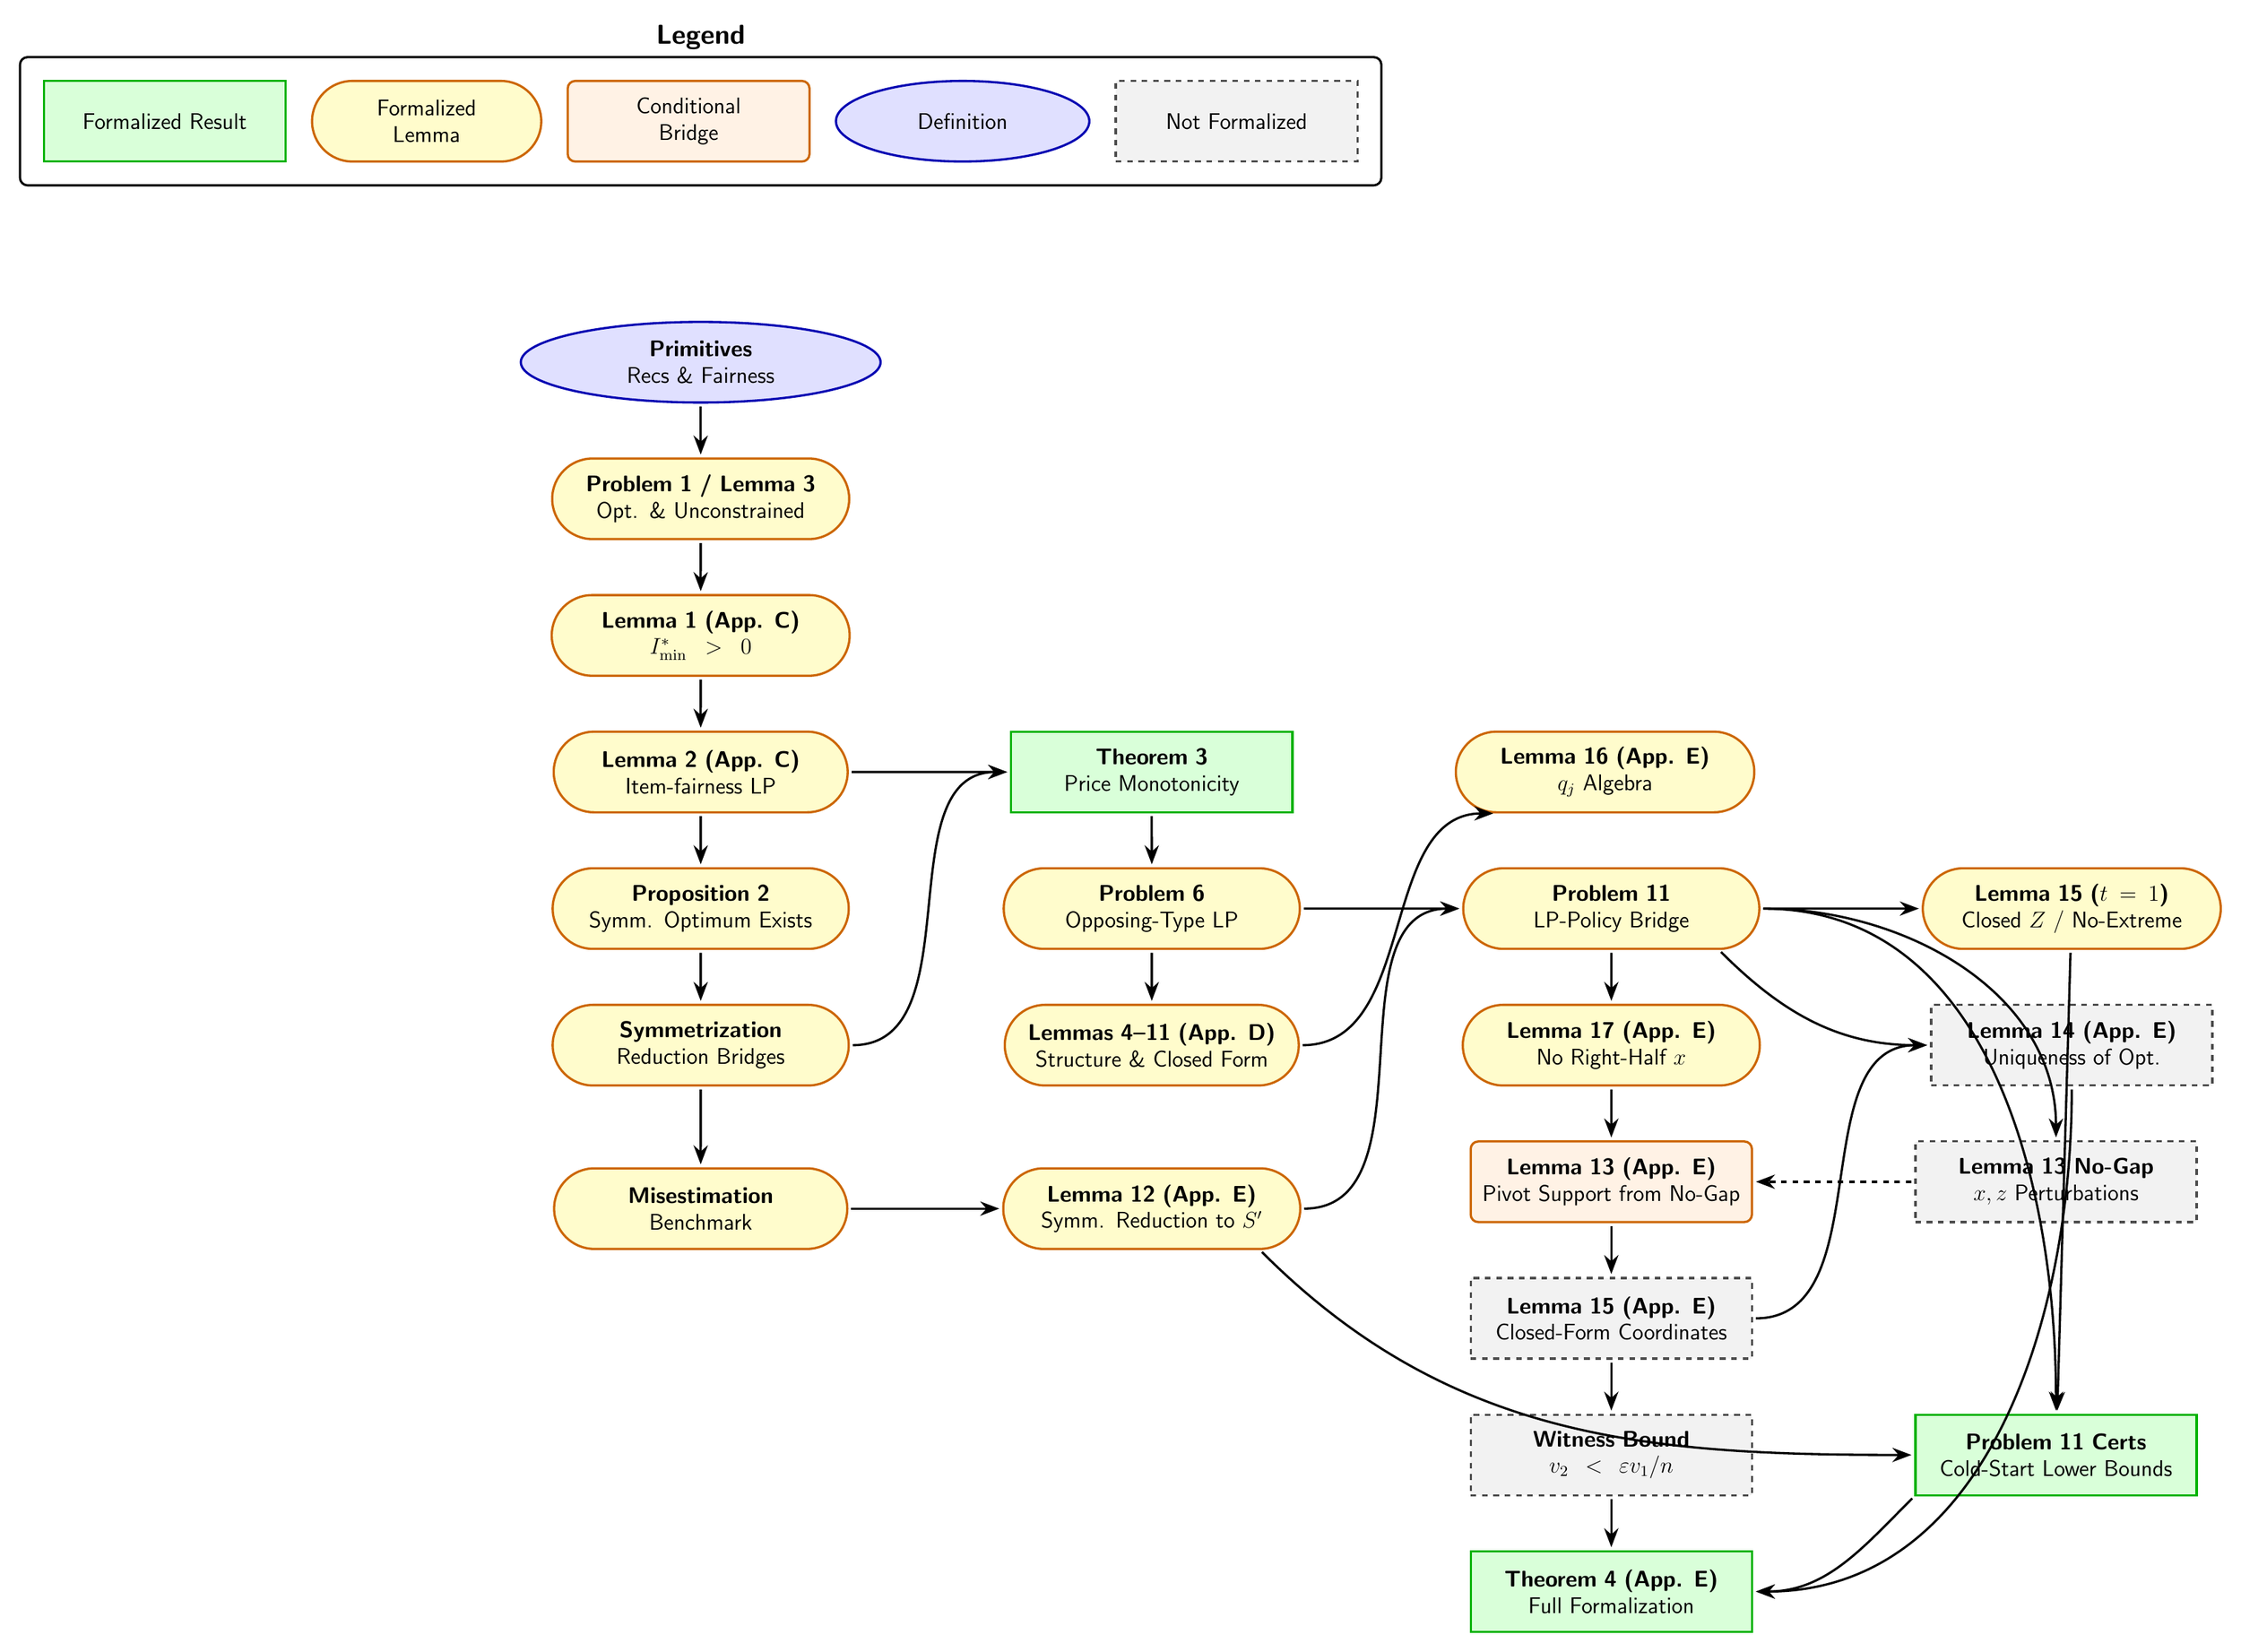
\begin{tikzpicture}

% --- Legend ---
\node[dag_result, text width=3.1cm] (legRes) {Formalized Result};
\node[dag_lemma, right=0.45cm of legRes, text width=3.1cm] (legLem) {Formalized Lemma};
\node[dag_conditional, right=0.45cm of legLem, text width=3.1cm] (legCond) {Conditional Bridge};
\node[dag_model, right=0.45cm of legCond, text width=3.1cm] (legDef) {Definition};
\node[dag_unformalized, right=0.45cm of legDef, text width=3.1cm] (legOpen) {Not Formalized};
\daglegend{(legRes)(legLem)(legCond)(legDef)(legOpen)}{Legend}

% --- Column 1 (Primitives & Symmetric Reduction) ---
\node[dag_model, below=2.5cm of Legend] (BaseDefs) {\textbf{Primitives} \\ Recs \& Fairness};
\node[dag_lemma, below=1cm of BaseDefs] (Prob1) {\textbf{Problem 1 / Lemma 3} \\ Opt. \& Unconstrained};
\node[dag_lemma, below=1cm of Prob1] (Lemma1) {\textbf{Lemma 1 (App. C)} \\ $I^*_{\min} > 0$};
\node[dag_lemma, below=1cm of Lemma1] (Lemma2) {\textbf{Lemma 2 (App. C)} \\ Item-fairness LP};
\node[dag_lemma, below=1cm of Lemma2] (Prop2) {\textbf{Proposition 2} \\ Symm. Optimum Exists};
\node[dag_lemma, below=1cm of Prop2] (SymmRed) {\textbf{Symmetrization} \\ Reduction Bridges};
\node[dag_lemma, below=1.5cm of SymmRed] (BaseMis) {\textbf{Misestimation} \\ Benchmark};

% --- Column 2 (Theorem 3 & Problem 6) ---
\node[dag_result, right=of Lemma2] (Thm3a) {\textbf{Theorem 3} \\ Price Monotonicity};
\node[dag_lemma, below=1cm of Thm3a] (Prob6) {\textbf{Problem 6} \\ Opposing-Type LP};
\node[dag_lemma, below=1cm of Prob6] (Lemmas4to11) {\textbf{Lemmas 4--11 (App. D)} \\ Structure \& Closed Form};
\node[dag_lemma, below=1.5cm of Lemmas4to11] (Lemma12) {\textbf{Lemma 12 (App. E)} \\ Symm. Reduction to $S'$};

% --- Column 3 (Problem 11 & Theorem 4) ---
\node[dag_lemma, right=of Prob6] (Problem11Core) {\textbf{Problem 11} \\ LP-Policy Bridge};
\node[dag_lemma, below=1cm of Problem11Core] (Lemma17) {\textbf{Lemma 17 (App. E)} \\ No Right-Half $x$};
\node[dag_conditional, below=1cm of Lemma17] (Lemma13) {\textbf{Lemma 13 (App. E)} \\ Pivot Support from No-Gap};
\node[dag_unformalized, right=of Lemma13] (NoGap) {\textbf{Lemma 13 No-Gap} \\ $x,z$ Perturbations};
\node[dag_unformalized, below=1cm of Lemma13] (Lemma15) {\textbf{Lemma 15 (App. E)} \\ Closed-Form Coordinates};
\node[dag_unformalized, below=1cm of Lemma15] (VExist) {\textbf{Witness Bound} \\ $v_2 < \varepsilon v_1 / n$};
\node[dag_result, below=1cm of VExist] (Theorem4Final) {\textbf{Theorem 4 (App. E)} \\ Full Formalization};

% --- Column 4 (Extras) ---
\node[dag_lemma, right=of Thm3a] (Lemma16) {\textbf{Lemma 16 (App. E)} \\ $q_j$ Algebra};
\node[dag_lemma, right=of Problem11Core] (PivotOne) {\textbf{Lemma 15 ($t=1$)} \\ Closed $Z$ / No-Extreme};
\node[dag_unformalized, below=1cm of PivotOne] (Lemma14) {\textbf{Lemma 14 (App. E)} \\ Uniqueness of Opt.};
\node[dag_result, right=of VExist] (Theorem4Part) {\textbf{Problem 11 Certs} \\ Cold-Start Lower Bounds};

% --- Edges ---
\draw[dag_arrow] (BaseDefs) -- (Prob1);
\draw[dag_arrow] (Prob1) -- (Lemma1);
\draw[dag_arrow] (Lemma1) -- (Lemma2);
\draw[dag_arrow] (Lemma2) -- (Prop2);
\draw[dag_arrow] (Prop2) -- (SymmRed);
\draw[dag_arrow] (SymmRed) -- (BaseMis);

\draw[dag_arrow] (Lemma2) -- (Thm3a);
\draw[dag_arrow] (SymmRed.east) to[out=0, in=180] (Thm3a.west);
\draw[dag_arrow] (Thm3a) -- (Prob6);
\draw[dag_arrow] (Prob6) -- (Lemmas4to11);
\draw[dag_arrow] (BaseMis.east) to[out=0, in=180] (Lemma12.west);

\draw[dag_arrow] (Lemmas4to11.east) to[out=0, in=180] (Lemma16.south west);
\draw[dag_arrow] (Prob6) -- (Problem11Core);
\draw[dag_arrow] (Lemma12.east) to[out=0, in=180] (Problem11Core.west);

\draw[dag_arrow] (Problem11Core) -- (Lemma17);
\draw[dag_arrow] (Lemma17) -- (Lemma13);
\draw[dag_arrow] (Problem11Core.east) to[out=0, in=90] (NoGap.north);
\draw[dag_dashed_arrow] (NoGap) -- (Lemma13);
\draw[dag_arrow] (Lemma13) -- (Lemma15);
\draw[dag_arrow] (Lemma15) -- (VExist);
\draw[dag_arrow] (VExist) -- (Theorem4Final);

\draw[dag_arrow] (Problem11Core) -- (PivotOne);
\draw[dag_arrow] (Problem11Core.south east) to[out=315, in=180] (Lemma14.west);
\draw[dag_arrow] (Lemma15.east) to[out=0, in=180] (Lemma14.west);

\draw[dag_arrow] (Lemma12.south east) to[out=315, in=180] (Theorem4Part.west);
\draw[dag_arrow] (Problem11Core.east) to[out=0, in=90] (Theorem4Part.north);
\draw[dag_arrow] (PivotOne) -- (Theorem4Part);

\draw[dag_arrow] (Theorem4Part.south west) to[out=225, in=0] (Theorem4Final.east);
\draw[dag_arrow] (Lemma14.south) to[out=270, in=0] (Theorem4Final.east);

\end{tikzpicture}
\end{document}
